\section{Django - Introduction}

\par{Django is a web framework which makes building web apps simpler and faster,
by providing:}

\begin{enumerate}
	\item[]{a division between logic and presentation components}
	\item[]{auto-generation of web admin}
	\item[]{many APIs for common tasks}
	\item[]{extra URL mapping control \mymarginpar{URL-Django-HTML vs URL-HTML}}
\end{enumerate}

\subsection{Design Philosophy}

	\par{Django follows the \ita{loose coupling} principle, which states that
different layers of the app should not know about each other's details ; and the
\ita{DRY} principle which states that \ita{"Every piece of knowledge must have a single, unambiguous, authoritative
representation within a system"}, i.e one should know exactly where to lookup
required data without having to repeat it in logically separate modules}

\subsection{Essential (pre-packaged) Modules}

\begin{itemize}
	\item[]{Create Read Update Delete Admin Interface}
	\item[]{Authorization Systems}
	\item[]{Form, Session Handling}
	\item[]{Syndication Awareness (e.g. RSS)}
	\item[]{Caching}
	\item[]{Internationalization}
\end{itemize}

\subsection{MVT}

\defn{ORM}{a programming technique for converting data of different types using
OO concepts and languages}

\par{Django uses a variant of the
\href{https://blog.codinghorror.com/understanding-model-view-controller/}{MVC}
design pattern - \ita{MVT}.The Model-View-Template is a \ita{data-driven} framework which separates
an app into the following logical units}

\begin{enumerate}
	\item{\textbf{Models : } is an abstraction of the database, where data
structures are represented via python objects}

	\par{This abstraction is achieved via \ita{Object Relational Mapping} ,
where one can query the database via the usual object dot access notation, and
Django in the background, converts both the objects and our queries into valid
SQL (or whatever DB language the project is using)}

	\item{\textbf{Views : } provide both the representation logic and app logic.
It's here that one handles HTTP requests/responses via response objects. It
is also here than one can query data via
the models' API, where a template populated with results is returned for
presenting}
	\item{\textbf{Templates : } provide the presentation layout (decoupled from
the data), composed of
static HTML, with the possibility of using the \ita{django template language} to
include some dynamic elements}
\end{enumerate}

	\begin{figure}[H]
		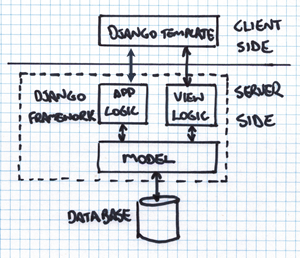
\includegraphics{mvt.png}
		\caption{\href{https://djangobook.com/mdj2-django-structure/}{Django
MVT}}
	\end{figure}

 \rem{Views are not queried directly via the client, instead the urls.py file
allows for finer control, pairing a given URL (or URL pattern) to a certain
view.}


